\documentclass[default]{beamer}
\setbeamertemplate{navigation symbols}{}

\usetheme{Frankfurt}
%\useoutertheme{infolines}
\usecolortheme{beaver}

\usepackage[utf8]{inputenc}					% Выбор языка и кодировки
\usepackage[english, russian]{babel}	% Языки: русский, английский
\usepackage{csquotes}

\usepackage{tikz}
\usetikzlibrary{arrows,shapes,calc}
\everymath{\displaystyle}
\tikzstyle{every picture}+=[remember picture]

\usepackage{animate}
\usepackage{fp}
\usepackage{textpos}
\usepackage{multimedia}
\usepackage{media9}
\usepackage{listings}
\usepackage{minted}

\graphicspath{{../../images/}} 			% Пути к изображениям

\makeatletter
\setbeamertemplate{footline}
{
	\leavevmode%
	\hbox{%
		\begin{beamercolorbox}[wd=.333333\paperwidth,ht=2.25ex,dp=1ex,center]{author
				in head/foot}%
			\usebeamerfont{author in
				head/foot}\insertshortauthor~~\beamer@ifempty{\insertshortinstitute}{}{(\insertshortinstitute)}
		\end{beamercolorbox}%
		\begin{beamercolorbox}[wd=.333333\paperwidth,ht=2.25ex,dp=1ex,center]{title in
				head/foot}%
			\usebeamerfont{title in head/foot}\insertshorttitle
		\end{beamercolorbox}%
		\begin{beamercolorbox}[wd=.333333\paperwidth,ht=2.25ex,dp=1ex,right]{date in
				head/foot}%
			\usebeamerfont{date in head/foot}\insertshortdate{}\hspace*{2em}
			\insertframenumber{}\hspace*{2ex} 
		\end{beamercolorbox}
	}%
	\vskip0pt%
}


\begin{document}
	
	\title[РобоНИС]{НИС: методы искусственного интеллекта в робототехнике}
	\author[Панов, Яковлев]{\textbf{Александр Панов и Константин Яковлев}}
	\institute[ВШЭ]{НИУ ВШЭ}
	\date{4 декабря 2017} 
	
	{
	\setbeamertemplate{headline}{}
	\begin{frame}
		
		\titlepage
		\centering
		\href{mailto:apanov@hse.ru}{apanov@hse.ru}
		
		
\includegraphics[width=25pt]{misc/logos/hse.png} \hspace{10pt}
		\includegraphics[width=100pt]{misc/logos/ras.png} \hspace{10pt}
		
\includegraphics[width=80pt]{misc/logos/frccsc.png}
		
	\end{frame}
	}	

	\section{Психология в ИИ}
	\subsection{1}

	\begin{frame}
		\frametitle{Когнитивные архитектуры}
		\begin{center}
			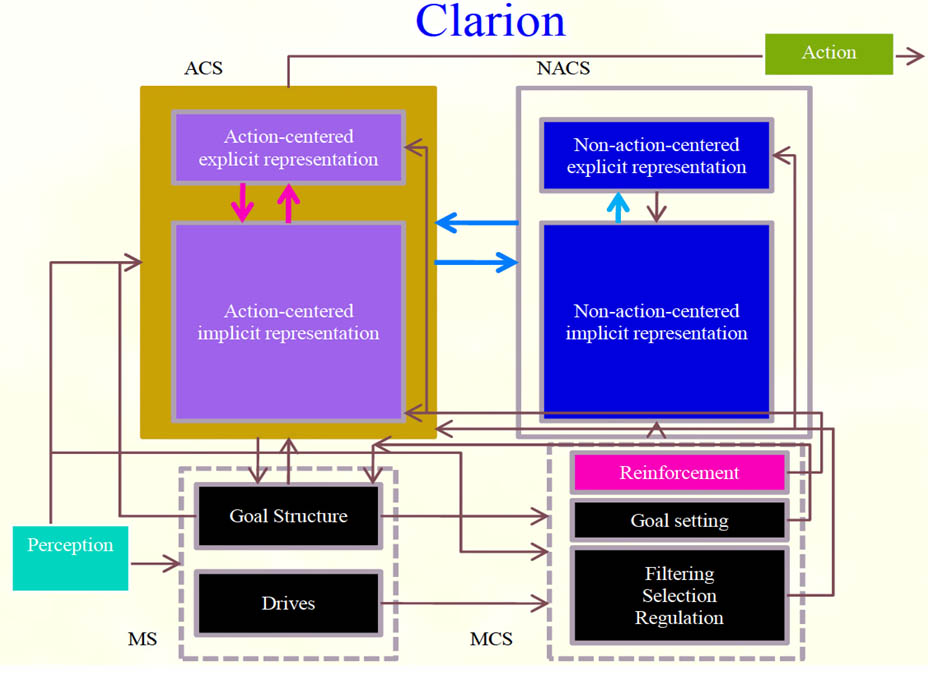
\includegraphics[width=0.3\textwidth]{agent-schemas/en/clarion.jpg}
			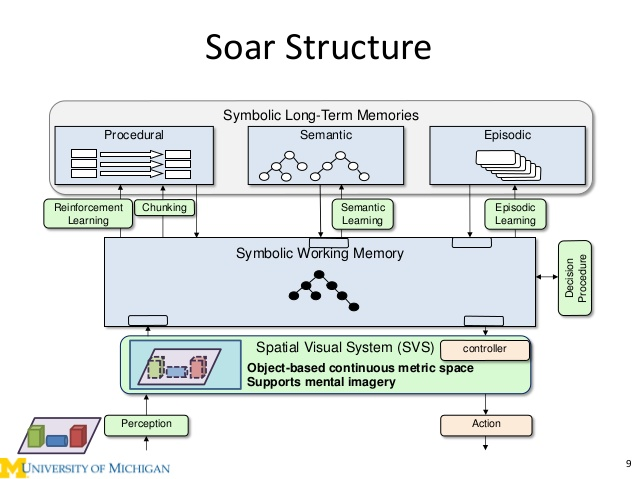
\includegraphics[width=0.3\textwidth]{agent-schemas/en/soar.jpg}
		\end{center}
		\scriptsize
		Недостатки современных когнитивных архитектур:
		\begin{itemize}
			\item Концептуальная нерешенность проблемы привязки символов (symbol grounding problem) - CLARION
			\item Отсутствие деятельностной модели поведения системы - реализация только некоторых когнитивных аспектов
			\item Иерархичность представления знаний (4D/RCS)
			\item Возможность реализации иерархического планирования
			\item Реализация обучения концептуальным знаниям - Cognitive Mario
			\item Моделирование рефлексивного поведения
		\end{itemize}

	\end{frame}

	
	\begin{frame}
		\frametitle{Когнитивные науки}
		
		
		\centering
		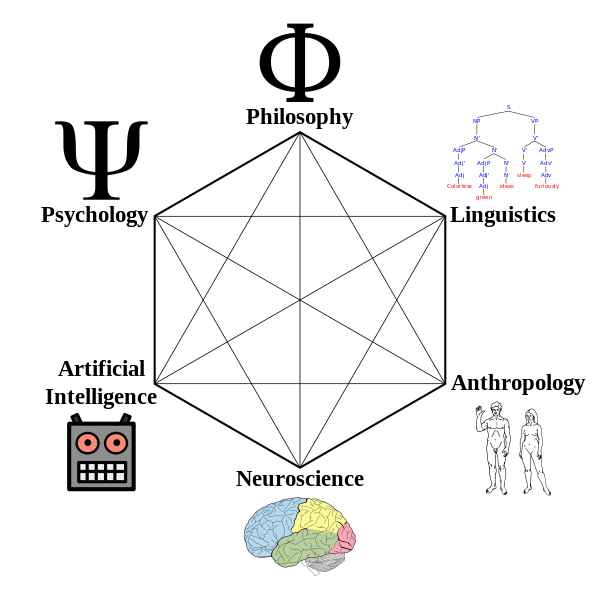
\includegraphics[width=0.5\textwidth]{misc/psycho/cogsci.png}
		
		Когнитивная наука (лат. cognitio <<познание>>) - междисциплинарное научное направление изучающее психику, разум (mind) человека и реализующие его процессы.
	\end{frame}	

	\begin{frame}
		\frametitle{Культурно-исторический подход}
		\small
		\begin{columns}
			\begin{column}{0.4\textwidth}
				\includegraphics[width=0.8\textwidth]{misc/psycho/activity.pdf}			
			\end{column}
			\begin{column}{0.6\textwidth}
				\begin{center}
					\includegraphics[width=0.17\textwidth]{misc/photos/leontyev.jpg}
				\end{center}
				Основные положения:
				\begin{itemize}
					\item Поведение человека - это двойная иерархическая структура мотивы-цели и действия-операции.
					\item Деятельность – это активный, целенаправленный процесс.
					\item Действия человека предметны; их цели носят социальный характер.
					\item Сознание и деятельность неразрывно связаны.
				\end{itemize}
			\end{column}
		\end{columns}
	\end{frame}

	\begin{frame}
		\frametitle{Знак как орудие психической деятельности}
		\begin{center}
			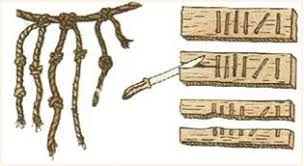
\includegraphics[width=0.4\textwidth]{misc/psycho/link.jpg}
		\end{center}
		
		\begin{itemize}
			\item Знак - это искусственно созданный человеком стимул, средство для управления своим поведение и поведением других.
			\item История развития человечества - это история развития знака: чем более развита система знаков в поколении, тем более развиты высшие психические функции.
			\item Знаки: наскальный рисунок, приметы, жесты, речь, ноты и т.д.
		\end{itemize}
	\end{frame}

	\begin{frame}
		\frametitle{Прикладная семиотика}
		\begin{center}
			\includegraphics[width=0.2\textwidth]{signs/ru/sign-frame.png}
		\end{center}
		\vspace{-15pt}
		\scriptsize
		Семиотические базы знаний:
		\begin{itemize}
			\item \textbf{Именованность}: информационная единица, которая претендует на то, чтобы называться знанием, должна иметь некоторую собственную метку - имя.акс
			\item \textbf{Структурированность}: информационная единица должна обладать своей внутренней структурой.
			\item \textbf{Принцип матрешки}: знаки за счет связей наследования как бы вкладываются друг в друга, обеспечивая описание сущностей на различных уровнях.
			\item \textbf{Связность}: знаки благодаря различным отношениям объединяются в сеть.
			\item \textbf{Активность}: в сетях знаков становится возможной реализация принципа <<активизация знаний - источник активизации процедур>>.
			\item \textbf{Рефлексивность}: появление метауровня позволяет системе рассуждать о самой себе, о характере имеющейся у нее информации об окружающем мире.
		\end{itemize}
		
	\end{frame}

	\begin{frame}
		\frametitle{Картина мира субъекта деятельности}
		\scriptsize
		\onslide<1->{
			Картина мира субъекта деятельности - это представления субъекта о внешней среде, о своих собственных характеристиках, целях, мотивах, о других субъектах и операции (произвольные и непроизвольные), осуществляемые на основе этих представлений.
		}
		\onslide<2->{
			\par\smallskip
			Элементом картины мира является знак:
			\begin{itemize}
				\item в смысле культурно-исторического подхода Выготского-Лурии,
				\item выполняющий функции в соответствии с теорией деятельности Леонтьева.
			\end{itemize}
		}
		\onslide<3->{
			\begin{columns}
				\begin{column}{0.4\textwidth}
					\centering
					\includegraphics[width=0.6\textwidth]{signs/ru/sign_color_book_ru}
				\end{column}
			}
			\onslide<4->{
				\begin{column}{0.6\textwidth}
					\begin{columns}
						\begin{column}{0.5\textwidth}
							\centering
							\includegraphics[width=\textwidth]{misc/phisio/ivan_cyrc}
						\end{column}
						\begin{column}{0.5\textwidth}
							\centering
							\includegraphics[width=\textwidth]{misc/phisio/workspace}
						\end{column}
					\end{columns}
					
				\end{column}
			\end{columns}
			В пользу существования такой структуры свидетельствуют:
			\begin{itemize}
				\item нейрофизиологические данные (Эдельман, Иваницкий, Маунткастл и др.),
				\item другие психологические теории (например, трехкомпонентная модель Станович).
			\end{itemize}
		}
	\end{frame}
		
	\begin{frame}
		\frametitle{Три образующих элемента картины мира}
		\footnotesize
		\begin{figure}
			\includegraphics[width=0.3\textwidth]{signs/ru/sign_colored}
		\end{figure}
		\vspace{-10pt}
		Представляемая сущность описывается тремя причинно-следственными (каузальными) структурами:
		\begin{itemize}
			\item {\color{red}структура образа} - представление взаимосвязи внешних сигналов и внутренних характеристик субъекта (агента) - сенсо-моторное представление,
			\item {\color{blue}структура значения} - обобщенное знание о соотношениях во внешнем мире, согласованное в некоторой группе субъектов (агентов),
			\item {\color{green!60!black}структура личностного смысла} - ситуационная потребностно-мотивационная интерпретация знаний о соотношениях во внешней среде (значение для себя).
		\end{itemize}
	\end{frame}
		
	\begin{frame}
		\frametitle{Уровни представления}
		\begin{figure}
		\includegraphics[width=0.7\textwidth]{signs/ru/sign_levels}
		\end{figure}
	\end{frame}

	\begin{frame}
		\frametitle{Каузальная матрица}                             
		\centering
		\includegraphics[width=0.7\textwidth]{causnet/caus_matr}
	\end{frame}

	\begin{frame}
		\frametitle{Каузальная сеть на образах}
		\footnotesize
		\textbf{Каузальная сеть} на множестве образов знаков $W_p=\langle V_p, E_p \rangle$ - помеченный ориентированный граф, в котором
		\begin{itemize}
			\item каждому узлу $v\in V_p$ ставится в соответствие кортеж казуальных матриц $Z^p(s)$ образа некоторого знака $s$ ($v\rightarrow Z^p(s)$);
			\item ребро $e=(v_1, v_2)$ принадлежит множеству ребер графа $E$, если $v_1\rightarrow Z^p(s_1), v_2\rightarrow Z^p(s_2)$ и $s_1\in S_p(s_2)$;
			\item каждому ребру графа $e=(v_1, v_2), v_1\rightarrow Z^p(s_1), v_2\rightarrow Z^p(s_2)$ ставится в соответствие метка $\epsilon=(\epsilon_1,\epsilon_2,\epsilon_3)$ - кортеж трех натуральных чисел:
			\begin{itemize}
				\item $\epsilon_1$ - индекс исходной матрицы в кортеже $Z^p(s_1)$, может принимать специальное значение 0, если исходными могут служить любые матрицы из кортежа;
				\item $\epsilon_2$ - индекс целевой матрицы в кортеже $Z^p(s_2)$, строка которой ставится в соответствие признаку $s_1$;
				\item $\epsilon_2$ - индекс столбца в целевой матрице, в которой в соответствующей признаку $s_1$ строке стоит 1, может принимать положительные значения (\textit{столбцы условий}) и отрицательные (\textit{столбцы эффектов}).
			\end{itemize}		
		\end{itemize}
	\end{frame}
		
	\begin{frame}
		\frametitle{Каузальная сеть на образах: пример}
		
		\centering
		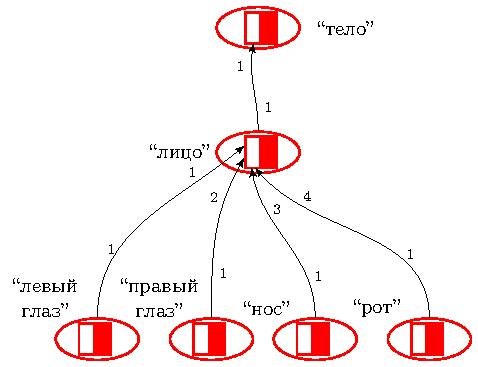
\includegraphics[page=1,width=0.6\textwidth]{examples/causnet/caus_net_colored}
		\includegraphics[width=0.4\textwidth]{misc/photos/face}
	\end{frame}
		
	\begin{frame}
		\frametitle{Каузальная сеть на значениях: пример}
		
		\begin{figure}
		\includegraphics[page=2,width=0.7\textwidth]{examples/causnet/caus_net_colored}
		\end{figure}
		
	\end{frame}
		
	\begin{frame}
		\frametitle{Каузальная сеть на личностных смыслах: пример}
		
		\begin{figure}
		\includegraphics[page=3,width=0.7\textwidth]{examples/causnet/caus_net_colored}
		\end{figure}
		
	\end{frame}	
	
	\section{Применение в робототехнике}
	\subsection{2}

	\begin{frame}
		\frametitle{Особенности постановки задачи}
		
		Рассматривается случай группового взаимодействия автономных технических объектов (агентов), в котором:
		\begin{itemize}
			\item агенты решают общую задачу (имеют общую цель высшего уровня),
			\item агенты действуют независимо друг от друга (децентрализованное управление), в т.ч. могут ставить индивидуальные подцели и достигать их,
			\item агенты обладают различными характеристиками, как техническими, так и когнитивными, т.е. разными стратегиями поведения,
			\item агенты обладают различными картинами мира,
			\item агенты действуют в меняющейся среде.
		\end{itemize}
		
	\end{frame}

	\begin{frame}
		\frametitle{Требования к представлению знаний}
		
		На представление пространственных и временных знаний в задаче согласованного перемещения с такими особенностями налагается ряд ограничений:
		\begin{itemize}
		\item необходимость поддержки некоторого протокола коммуникации, разделение знаний на коммуницируемые и некоммуницируемые (личные),
		\item необходимость выделения компоненты знания, не зависящей от индивидуальных (личных) характеристик агента,
		\item требование к наличию механизма связывания реальных объектов внешней среды и процедур их распознавания с символьным коммуницируемым представлением (symbol grounding problem),
		\item поддержка механизмов пополнения картины мира (обучение и абстрагирование).
		\end{itemize}
	\end{frame}

	\begin{frame}
		\frametitle{Практические задачи}
		
		\centering
		\includegraphics[width=\textwidth]{examples/signs/robotic_signs}
		
	\end{frame}

	\begin{frame}
		\frametitle{Задача интеллектуального перемещения}
		
		\begin{columns}
		\begin{column}{0.55\textwidth}
		\begin{center}
		\includegraphics[page=1,width=0.8\textwidth]{examples/plan/slides_colored}
		\end{center}
		\vspace{-7pt}
		\small
		\textbf{Задача}
		
		Целевая область не достижима некоторым агентом самостоятельно (с использованием только методов планирования траектории).
		
		\textbf{Решение}
		
		Агенты должны поддерживать коммуникацию и модифицировать свои собственные планы с учетом коалиционных подзадач.
		
		\end{column}
		\begin{column}{0.45\textwidth}
		Особенности:
		\begin{itemize}
		\item Меняющаяся внешняя среда.
		\item Различные типы препятствий (некоторые могут быть разрушены).
		\item Агенты обладают различной функциональностью.
		\item Общая пространственная цель (ВСЕ агенты должны достичь определенной области на карте).
		\end{itemize}
		\end{column}
		\end{columns}
	\end{frame}

	\begin{frame}
		\frametitle{Представление пространственных знаний}
	
		\includegraphics[width=\textwidth]{examples/representations/rita_ex_proc.png}
	
	\end{frame}

	\begin{frame}
		\frametitle{Представление пространственных знаний}
	
		\includegraphics[width=\textwidth]{examples/representations/bica_psy_path.png}

	\end{frame}	

	\begin{frame}
		\frametitle{Представление действий по перемещению}
		
		Действия по перемещению "--- знаки $s_t$ (признаки $f_t$, $t$ "--- тип перемещения), которым соответствуют каузальные матрицы типа $Z_t$, состоящие из трёх столбцов 
		\[
		z_1=(l_x, I), z_2=(l_y, d_u, E), z_3=(l_y, I, t_v),
		\]
		где 
		\begin{itemize}
		\item $l_x$, $l_y$ "--- признаки, соответствующие категории расстояния в пространственной логике  (например, вплотную, близко, далеко и др.), 
		\item $d_u$ "--- признак, соответствующий категории направления в пространственной логике (например, впереди, слева и др.), 
		\item $t_v$ "--- признак, соответствующий категории времени во временной логике (например, скоро, в будущем и др.),
		\item $I$ "--- признак присутствия самого агента, 
		\item $E$ "--- признак отсутствия препятствия.
		\end{itemize}
	\end{frame}	

	\begin{frame}
		\frametitle{Распределение ролей при решении задачи}
		\begin{center}
		\scalebox{0.7}{
		\animategraphics{12}{examples/plan/slides_colored}{}{}			
		}
		\end{center}
	\end{frame}

	\begin{frame}
		\frametitle{Пример по перемещению}
		
		\begin{center}
		\includegraphics[page=1,width=0.85\textwidth]{examples/plan/slides_colored}
		\end{center}
		\par\bigskip
		Актуализированные знаки агента $A_1$: ``область $X_6$'', ``далеко'', ``перемещение 1'' $\rightarrow$ \color{green!70!black} операции планирования траектории.
	\end{frame}

	\begin{frame}
		\frametitle{Пример по перемещению}
		
		\begin{center}
		\includegraphics[page=31,width=0.85\textwidth]{examples/plan/slides_colored}
		\end{center}
		\par\bigskip
		Актуализированные знаки агента $A_1$: ``препятствие 1'', ``рядом'', ``область $X_6$''.
	\end{frame}
	
	\begin{frame}
		\frametitle{Пример по перемещению}
	
		\begin{center}
		\includegraphics[page=42,width=0.85\textwidth]{examples/plan/slides_colored}
		\end{center}
		\par\bigskip
		Актуализированные знаки агента $A_1$: ``отправить сообщение'', ``агент $A_2$''.
	\end{frame}
	
	\begin{frame}
		\frametitle{Пример по перемещению}
		
		\begin{center}
		\includegraphics[page=58,width=0.85\textwidth]{examples/plan/slides_colored}
		\end{center}
		\par\bigskip
		Актуализированные знаки агента $A_2$: ``область $Y_3$'', ``далеко'', ``перемещение 2'' $\rightarrow$ \color{green!70!black} операции планирования траектории.
	\end{frame}
	
	\begin{frame}
		\frametitle{Пример по перемещению}
		
		\begin{center}
		\includegraphics[page=95,width=0.85\textwidth]{examples/plan/slides_colored}
		\end{center}
		\par\bigskip
		Актуализированные знаки агента $A_2$: ``область $Y_1$'', ``рядом'', ``препятствие 1'', ``разрушить''.
	\end{frame}
	
	\begin{frame}
		\frametitle{Пример по перемещению}
		
		\begin{center}
		\includegraphics[page=116,width=0.85\textwidth]{examples/plan/slides_colored}
		\end{center}
		\par\bigskip
		Актуализированные знаки агента $A_1$ and $A_2$: ``далеко'', ``перемещение 3'' $\rightarrow$ \color{green!70!black} операции планирования траектории.
	\end{frame}
	
	\begin{frame}
		\frametitle{Пример по перемещению}
		
		\begin{center}
		\includegraphics[page=171,width=0.85\textwidth]{examples/plan/slides_colored}
		\end{center}
		\par\bigskip
		Актуализированные знаки агента $A_1$ и $A_2$: целевое состояние (``область $G$'').
	\end{frame}


	\begin{frame}
		\frametitle{Знаки Я и Они в алгоритме планирования MAP}
		
		\begin{center}
		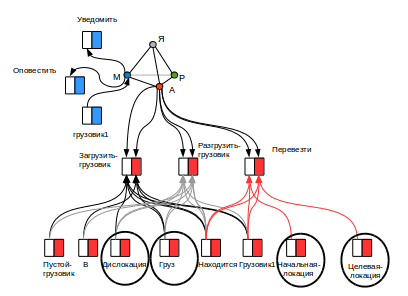
\includegraphics[width=0.6\textwidth]{sign-schemas/I-sign.png}
		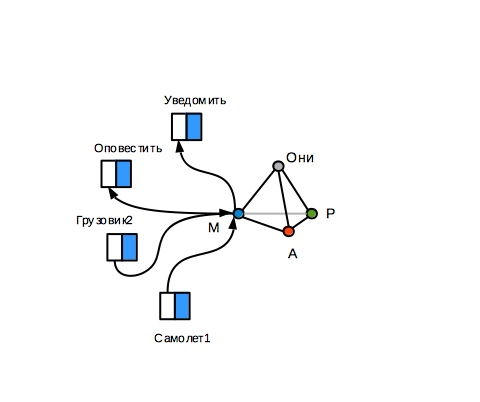
\includegraphics[width=0.5\textwidth]{sign-schemas/they-sign.png}
		\end{center}

	\end{frame}

	\begin{frame}
		\frametitle{Применение для решения интеллектуальных задач}
		\vspace{-5pt}
		\footnotesize
		\begin{columns}
		\begin{column}{0.5\textwidth}
		\begin{itemize}
		\item Моделирование внимания.
		\item Образование нового знания (концепта).
		\item Планирование поведения.
		\item Построение картины мира субъекта на основе текстов.
		\item Генерация сообщений на основе картин мира определенного типа (виртуальные ассистенты).
		\item Построение многоуровневых архитектур управления.
		\end{itemize}
		
		\end{column}
		\begin{column}{0.35\textwidth}
		\includegraphics[width=\textwidth]{agent-schemas/ru/architecture}
		\end{column}
		\begin{column}{0.15\textwidth}
		\includegraphics[width=\textwidth]{agent-schemas/ru/iagent}
		\end{column}
		
		\end{columns}

	\end{frame}

		

\end{document}
	
	
